%%%%%%%%%%%%%%%%%%%%%%%%%%%%%%%%%%%%%%%%%%%%%%%%%%%%%%%
% A template for Wiley article submissions.
% Developed by Overleaf. 
%
% Please note that whilst this template provides a 
% preview of the typeset manuscript for submission, it 
% will not necessarily be the final publication layout.
%
% Usage notes:
% The "blind" option will make anonymous all author, affiliation, correspondence and funding information.
% Use "num-refs" option for numerical citation and references style.
% Use "alpha-refs" option for author-year citation and references style.

\documentclass[alpha-refs]{wiley-article-05g}
% \documentclass[blind,num-refs]{wiley-article}

% Add additional packages here if required
\usepackage{siunitx}

% For figures
\usepackage{graphics}

%For captions - even though template has complex caption commands
\usepackage[labelfont=bf,justification=centering]{caption}
\usepackage[font=small,labelfont=bf]{subcaption}
\captionsetup[sub]{font=tiny,labelfont={bf,sf}}

%% For figures numbered by section
\usepackage{chngcntr}
\counterwithin{figure}{section}
\counterwithin{table}{section}

%% Additional links for hyperref
\usepackage[unicode=true,pdfusetitle,
 bookmarks=false,bookmarksnumbered=false,bookmarksopen=true,bookmarksopenlevel=2,
 breaklinks=false,pdfborder={0 0 1},backref=false,colorlinks=false]
 {hyperref}
\hypersetup{pdfstartview={XYZ null null 1}}

\usepackage[backend=bibtex,
			natbib=true, 
			style=chicago-authordate]{biblatex}
\addbibresource{Returns.bib}

\usepackage{array}
\usepackage{longtable}
%\usepackage{fullpage}

\usepackage{lmodern}
\newcommand{\graph}[3]{
\raisebox{-#1mm}{\includegraphics[height=#2em,width=3cm]{#3}}
}

\usepackage{booktabs} % for vertically partitioned table

\usepackage{lipsum}  % for fillers
\usepackage{float}

%% For landscape pages 

\usepackage{lscape}

%%%%%%%%#################################################################################%%%%%%%%%%%%%%%%%%%%%%%%%%%%%

% Update article type if known
\papertype{WORLD BANK EDUCATION GLOBAL PRACTICE}
% Include section in journal if known, otherwise delete
\paperfield{Russian Federation: Analytical Services and Advisory Activity: 
P170978}

\title{Returns to Education in the Russian Federation: Towards Evidence Based Decision Making with Social and Private Returns to Education}

% List acknowledgements here.
\fundinginfo{Thanks are due to the Ministry of Education and the Ministry of Finance for making the data available regarding graduate earnings and college and university income and expenditures. The code used for this paper is made freely available for all researchers at \url{https://bitbucket.org/zagamog/edreru/src/master/}}

% Include full author names and degrees, when required by the journal.
% Use the \authfn to add symbols for additional footnotes and present addresses, if any. Usually start with 1 for notes about author contributions; then continuing with 2 etc if any author has a different present address.

\author[*]{Ekaterina Melianova}
\author[*]{\hspace{-1em}Suhas Parandekar}
\author[*]{\hspace{-1em}Art\"{e}m Volgin}

% List abbreviations here, if any. Please note that it is preferred that abbreviations be defined at the first instance they appear in the text, rather than creating an abbreviations list.
\acks{\begin{normalsize}
\emph{Country Director:} Renaud Seligman; \emph{Regional Director:} Fadia Saadah; \emph{Practice Manager:} Harry Patrinos; \emph{Program Leader:} Dorota Nowak; \emph{Peer Reviewers}: Cristian Aedo; Ruslan Yemtsov; Husein Abdul-Hamid; \emph{Team members:} Polina Zavalina; Zhanna Terlyga. Thanks to seminar participants at the World Bank Moscow office on Jan. 29, 2020 for useful feedback. Any errors are a responsibility of the authors.
\end{normalsize}
\vspace{-0.2in}}

%\contrib[\authfn{1}]{Equally contributing authors.}

% Include full affiliation details for all authors
\affil[*]{Education Global Practice, Europe and Central Asia}

%\corraddress{Author One PhD, Department, Institution, City, State or Province, Postal Code, Country}
\corremail{sparandekar@worldbank.org}

%\presentadd[\authfn{2}]{Department, Institution, City, State or Province, Postal Code, Country}

% Include the name of the author that should appear in the running header
\runningauthor{P170978: WP05 - Private and Social Returns to Education}

\begin{document}

\maketitle

\begin{abstract}
This paper presents a preliminary analysis of a dataset distributed by the Ministry of Education of the Russian Federation that provides information on graduate salaries. The data is merged with information on income and fee revenue of colleges and universities to provide estimates of costs and benefits at an institutional level and private and social returns to education at a regional level. As the length of the data series on graduate earnings will grow over time, the estimates presented in this paper can be updated to provide sharper estimates of the costs and benefits of attending a particular institution.

% Please include a maximum of seven keywords
\keywords{Returns to Education, Higher Education, Cost-Benefit Analysis \emph{JEL Codes: I23, I26}}
\end{abstract}

\section{Description of Data}

The Ministry of Education provides information regarding  the salaries obtained by graduates and other related information at the website \hyperref[graduate.edu]{''http://graduate.edu.ru''}. A key purpose of this website is to provide accurate information to prospective university students and their families about the prospects of graduates from each of the universities or colleges. The Ministry of Finance collects information from all education establishments and others providing public service as a means to foster citizen engagement and accountability.This information includes details about revenue and income streams. This paper presents analysis from the merger of these two databases. The content of the data is presented in this section. Subsequent sections provide analysis and interpretation.

\subsection{Graduate.edu portal}

Graduate.edu allows the registered users to download all desirable information about the earnings of college or university graduates in .xlsx format. By using that service we obtained data about the number of graduates in 2013 in each university and college and their corresponding salaries in 2014, 2015 and 2016.
Our final set of data consists of 1909 colleges, 423 universities, and 2975 pairs of university-study areas with information about the graduates earning in them. We filtered out universities and colleges with less than 100 and 50 graduates in 2013, respectively. Salaries in 2014 and 2015 were adjusted to the prices of 2016.


\begin{table}[htbp!]
	\centering
	\begin{tabular}{rlllll}
		\hline
		& Mean & Std & Quantile.25. & Quantile.50. & Quantile.75. \\ 
		\hline
		College Graduates Avg. Earnings 2014 & 22,408 & 6,718 & 18,214 & 20,843 & 24,745 \\ 
		College Graduates Avg. Earnings 2015 & 21,036 & 6,243 & 17,172 & 19,611 & 23,375 \\ 
		College Graduates Avg. Earnings 2016 & 21,586 & 6,637 & 17,359 & 20,001 & 23,944 \\ 
		University Graduates Avg. Earnings 2014 & 34,910 & 15,282 & 24,811 & 30,481 & 40,376 \\ 
		University Graduates Avg. Earnings 2015 & 35,789 & 16,927 & 25,381 & 30,710 & 41,603 \\ 
		University Graduates Avg. Earnings 2016 & 36,937 & 18,353 & 25,410 & 31,692 & 42,500 \\ 
		\hline
	\end{tabular}
\end{table}



\begin{figure}[H]
	\centering
	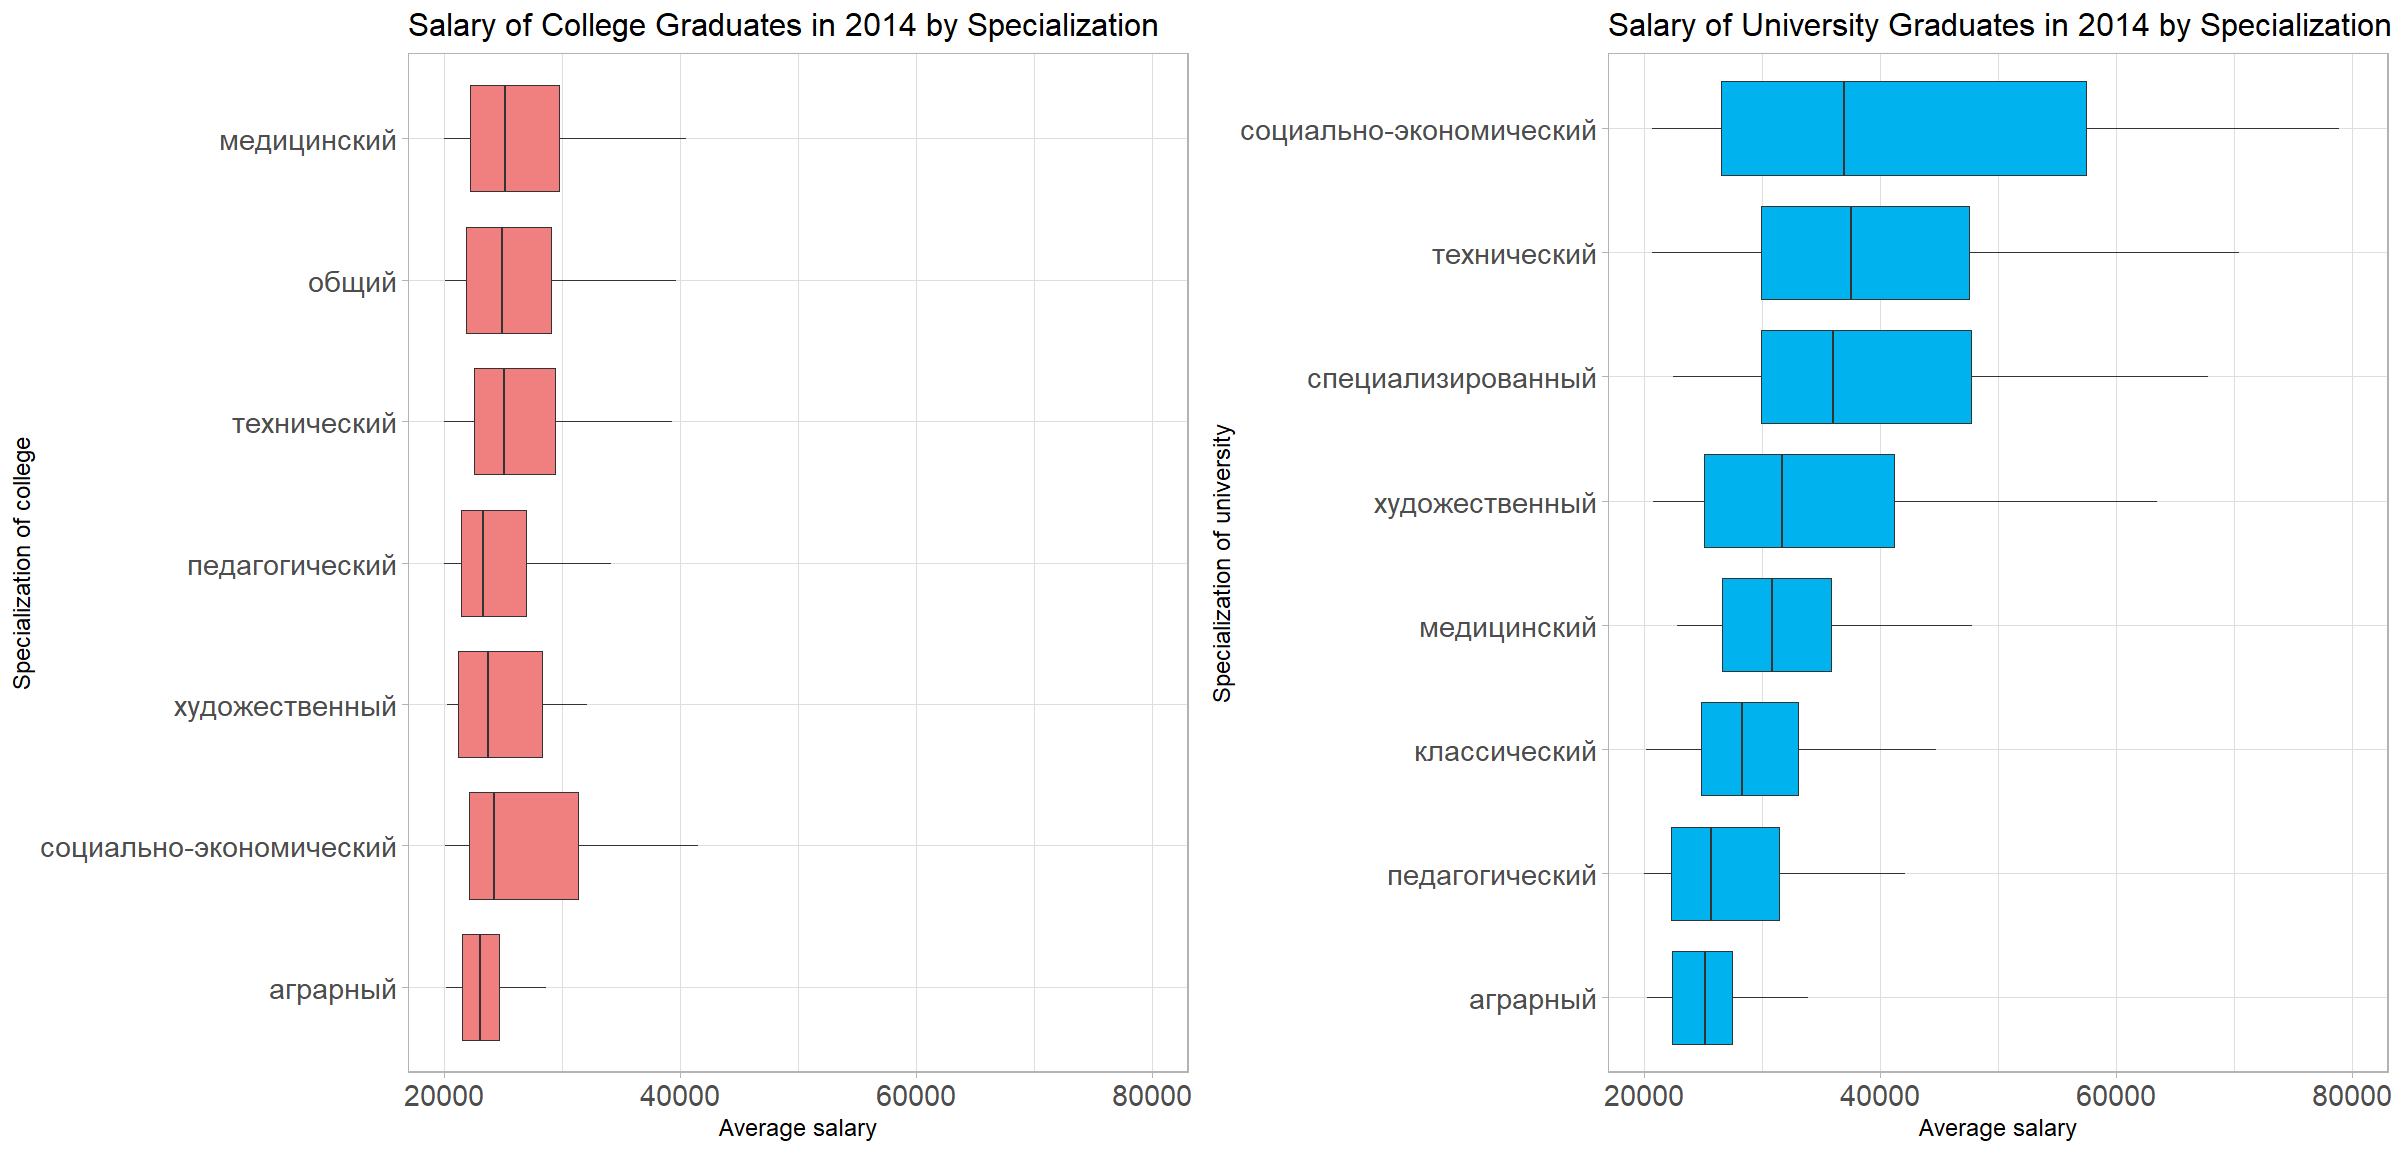
\includegraphics[width=400pt]{box_plot1a.png}
	\caption{Earnings in 2014 by Specialization}\label{fig:1.1}
\end{figure}

\newpage

\begin{figure}[H]
	\centering
	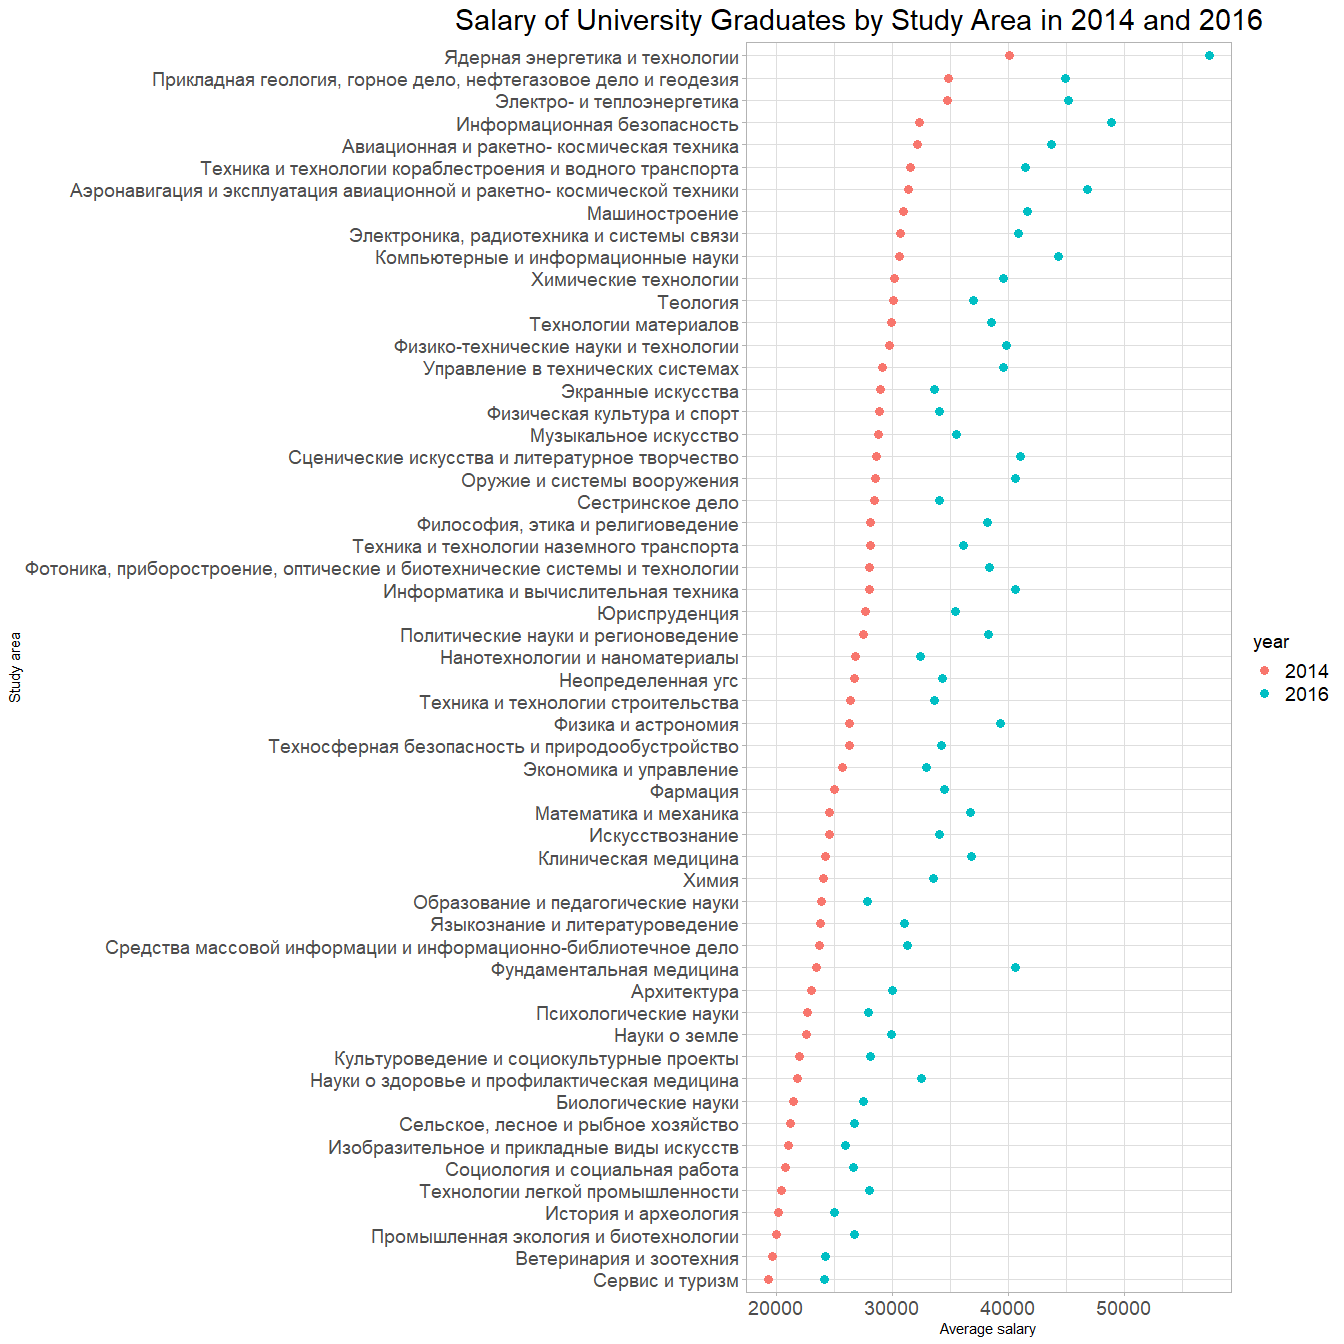
\includegraphics[width=400pt]{sal_inc.png}
	\caption{Earnings Growth 2014-16 by Specialization}\label{fig:1.2}
\end{figure}



\subsection{Bus.gov portal}

We obtained financial data about the colleges and universities from the open data section on the https://bus.gov.ru. It contains information about the total cash receipts of an organization for a given year and provides data on the income subcategories, such as cash receipts from paid services, target subsidy, budget investments, state (municipal) tasks. In our research, we approximated fee payments through the information about cash receipts from the paid services and used it together with the number of graduates for the calculation of the private education cost. To estimate the social cost of education we used total cash receipts in an organization. 

\begin{landscape}
\fontsize{9}{11}
\selectfont

\begin{table}[!htbp] \centering 
\renewcommand{\arraystretch}{1.0}
  \caption{Data regarding Tertiary Education Institutes} 
  \label{} 
\begin{tabular}{@{\extracolsep{1pt}}p{5cm}rrrrr} 
  		\hline
		& Mean & Std & Quantile.25. & Quantile.50. & Quantile.75. \\ 
		\hline
		Number of College Graduates in 2013 & 176 & 133 & 91 & 140 & 224 \\ 
		Total Cash Receipts in Colleges, mean 2012-2017 & 88,499,123 & 200,088,664 & 42,204,580 & 60,579,178 & 94,179,183 \\ 
		Cash Receipts from the Paid Services in Colleges, mean 2012-2017 & 12,004,525 & 24,174,679 & 3,338,267 & 6,714,013 & 13,290,758 \\ 
		Cash Receipts from the Target Subsidy in Colleges, mean 2012-2017 & 10,928,189 & 68,501,580 & 2,628,308 & 5,600,336 & 10,975,815 \\ 
		Cash Receipts from the Budget Investments in Colleges, mean 2012-2017 & 391,006 & 3,281,730 & 0 & 0 & 0 \\ 
		Cash Receipts from the State (Municipal) Tasks in Colleges, mean 2012-2017 & 62,185,103 & 78,598,657 & 31,545,198 & 45,165,347 & 68,748,188 \\ 
		Social Cost for Colleges & 209,009 & 376,700 & 107,376 & 149,017 & 224,786 \\ 
		Private Cost for Colleges & 22,515 & 26,853 & 8,606 & 16,156 & 28,189 \\ 
		Number of University Graduates in 2013 & 1,653 & 1,540 & 633 & 1,230 & 2,069 \\ 
		Total Cash Receipts in Universities, mean 2012-2017 & 1,584,286,956 & 2,428,205,237 & 483,322,825 & 852,711,495 & 1,554,176,934 \\ 
		Cash Receipts from the Paid Services in Universities, mean 2012-2017 & 635,645,477 & 1,093,170,696 & 131,150,223 & 296,913,560 & 687,080,404 \\ 
		Cash Receipts from the Target Subsidy in Universities, mean 2012-2017 & 219,245,816 & 307,653,669 & 71,807,802 & 128,997,272 & 220,246,527 \\ 
		Cash Receipts from the Budget Investments in Universities, mean 2012-2017 & 38,817,643 & 136,401,305 & 0 & 0 & 2,823,465 \\ 
		Cash Receipts from the State (Municipal) Tasks in Universities, mean 2012-2017 & 658,658,760 & 1,066,074,166 & 242,686,337 & 361,106,787 & 651,264,621 \\ 
		Social Cost for Universities & 272,584 & 282,826 & 107,101 & 176,603 & 308,564 \\ 
		Private Cost for Universities & 102,267 & 131,717 & 34,454 & 58,741 & 113,401 \\ 
		\hline
	\end{tabular}
\end{table}

\end{landscape}

\newpage

\section{Regional Estimates of Social and Private Returns}


In the first part of our research, we focus on calculating the social and private regional internal rate of return by using the following methodology. We utilize the average wage in each age from 2014 to 2018 Rosstat Survey to calculate the potential earnings profiles and then add the mean social and private cost estimates for the regions to the begging of that profile. We also adjust for the foregone earnings of graduates by adding to the educational cost the potential wage that graduates missed due to the enrollment in the university of college, we took average wage in the region as the approximation of such earnings.

Below you can see an estimate of social and private IRR of university graduates by regions of Russia. Both types of returns have high dispersion across the country: from around 40\% IRR in Magadanskaya and Ulyanovskaya oblast to the less than 15\% in Kurganskaya and Kurskaya oblast. It is interesting to notice that although Moscovskaya oblast has substantially high social and private returns, the Moscow lacking behind in that ranking with only 20\% of IRR. That may happen due to the circular migration from Moscovskaya Oblast to Moscow - people in Moscovskaya Oblast can get access to the cheaper education inside their region and still be able to work in the nearby capital.

\textbf{PLOT Social and Private Returns by region, Higher education}

The next graph demonstrates the social and private IRR of colleges. As you may notice the regional variation is still present, but not to the same extent as in universities - returns are lying between 20-30\% in most of the regions.

\textbf{PLOT Social and Private Returns by region, Vocational education}

The average levels of social returns of college and university graduates in a region are highly correlated - regions with a high level of university returns tend to have higher rates of college returns. Nonetheless, there are some exceptions: for example, Respublika Tatarstan has above average social returns of college graduates, but lacking behind in university returns. The situation in Sahalinskaya Oblast is directly the opposite - the region is characterized by one of the highest levels of social university returns, but the college returns are a lot lower than in most of the other regions. You can see a distribution of returns by two levels of education in the scatterplot below.

\textbf{PLOT Social Returns by regions}


\section{Institutional Returns for Colleges and Universities}

Data provided in graduate.edu allow us to calculate IRR directly for each educational organization. As in the previous part we use social and private cost as the cost part of the IRR specification, but now we utilize graduate salaries in 2014, 2015, and 2016 as the benefits obtained by the graduates. Resulting IRR estimations have a negative sign for most of the organizations since we have access only to the 3 years of observations after graduation. Although obtained results represent only short-run returns they still can be used to compare universities or colleges within each other.

Bellow, you can the tables with Top-10 and Bottom-10 universities and colleges ranked according to the level of social IRR.

\textbf{TOP/BOTTOM-10 universities}

\textbf{TOP/BOTTOM-10 college}

The provided data allow us to map the educational organizations according to their precise coordinates. We can observe a few examples of such plotting for Moscow universities and Saint Petersburg colleges with an indication of the level of social returns for each organization.

\textbf{PLOT Map Social IRR of universities in Moscow}

\textbf{PLOT Map Social IRR of colleges in Saint Petersburg}

Another aspect that can influence the rate of returns substantially is the education area of the organization. Technical specialization has the highest social internal return rate for both college and university and art specializations are amongst less returnable once for both educational levels. Medical universities in Russia, in opposite to their American counterparts, are also having one of the lowest internal return rates.

\textbf{PLOT Boxplots with social returns by specializations}

We estimate the factors which are explaining the difference in returns between organization by conducting 4 separate linear regression models with 1) Social IRR in colleges, 2) Private IRR in colleges, 3) Social IRR in universities, and 4) Private IRR in universities as dependent variables. We are going to use 1) the specialization of organization, 2) the number of graduates, 3) the number of staff, 4) the average wage in the organization, 5) the proportion of income obtained from paid services and 6) the average wage in the region as the main predictors for these models.

TODO




\newpage
\printbibliography

\end{document}
